
% This LaTeX was auto-generated from MATLAB code.
% To make changes, update the MATLAB code and republish this document.

\documentclass{article}
\usepackage{graphicx}
\usepackage{color}

\sloppy
\definecolor{lightgray}{gray}{0.5}
\setlength{\parindent}{0pt}

\begin{document}

    
    \begin{verbatim}
A_1=[2;-1;-1];
A_2=[-1;2;-1];
A_3=[-1;-1;2];

C_12 = cross(A_1,A_2);
C_31 = cross(A_3,A_1);
C_23 = cross(A_2, A_3);

C_12 = C_12/norm(C_12)
C_31 = C_31/norm(C_31)
C_23 = C_23/norm(C_23)

figure;
hold on;
grid on;

quiver3(0, 0, 0, A_1(1), A_1(2), A_1(3), 'r', 'LineWidth', 2, 'MaxHeadSize', 0.5);
quiver3(0, 0, 0, A_2(1), A_2(2), A_2(3), 'g', 'LineWidth', 2, 'MaxHeadSize', 0.5);
quiver3(0, 0, 0, A_3(1), A_3(2), A_3(3), 'b', 'LineWidth', 2, 'MaxHeadSize', 0.5);

quiver3(0, 0, 0, C_12(1), C_12(2), C_12(3), 'k', 'LineWidth', 2, 'MaxHeadSize', 0.5);

[X, Y] = meshgrid(-2:0.5:2, -2:0.5:2);
Z = (-C_12(1)*X - C_12(2)*Y) / C_12(3);

surf(X, Y, Z, 'FaceAlpha', 0.3, 'EdgeColor', 'none', 'FaceColor', 'cyan');

xlabel('X'); ylabel('Y'); zlabel('Z');
title('Vectors A1, A2, A3 and their Normal Vector');
legend('A1', 'A2', 'A3', 'Normal (C_{12})', 'Plane');

hold off;
axis equal;
view(3);
\end{verbatim}

        \color{lightgray} \begin{verbatim}
C_12 =

    0.5774
    0.5774
    0.5774


C_31 =

    0.5774
    0.5774
    0.5774


C_23 =

    0.5774
    0.5774
    0.5774

\end{verbatim} \color{black}
    
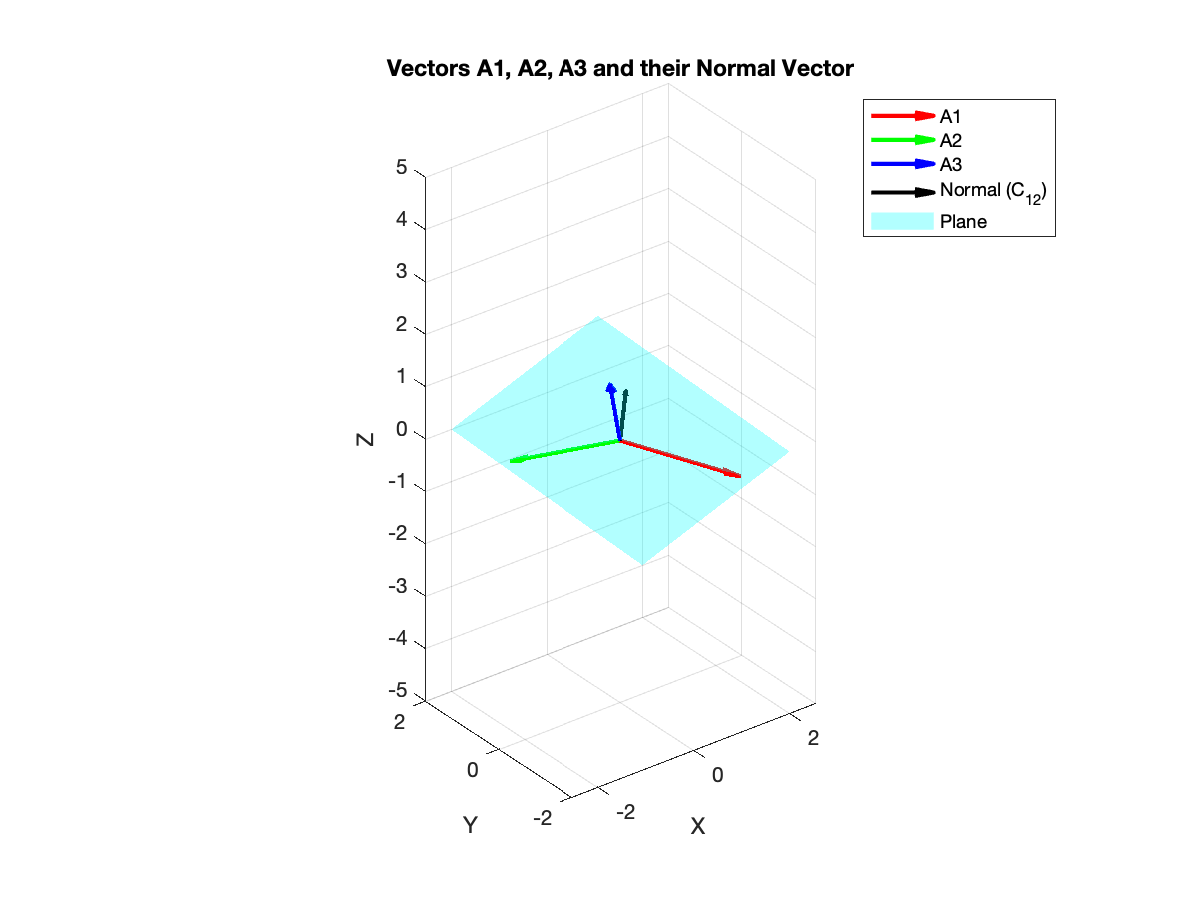
\includegraphics [width=4in]{untitled2_01.eps}



\end{document}

